\documentclass{bmvc2k}

\usepackage{amsmath}
\usepackage{amssymb}

%% Enter your paper number here for the review copy
% \bmvcreviewcopy{??}

\title{Author Guidelines for the\\ British Machine Vision Conference}

% Enter the paper's authors in order
% \addauthor{Name}{email/homepage}{INSTITUTION_CODE}
\addauthor{Susan Student}{http://www.vision.inst.ac.uk/~ss}{1}
\addauthor{Petra Prof}{http://www.vision.inst.ac.uk/~pp}{1}
\addauthor{Colin Collaborator}{colin@collaborators.com}{2}

% Enter the institutions
% \addinstitution{Name\\Address}
\addinstitution{
 The Vision Institute\\
 University of Borsetshire\\
 Wimbleham, UK
}
\addinstitution{
 Collaborators, Inc.\\
 123 Park Avenue,\\
 New York, USA
}

\runninghead{Student, Prof, Collaborator}{BMVC Author Guidelines}

% Any macro definitions you would like to include
% These are not defined in the style file, because they don't begin
% with \bmva, so they might conflict with the user's own macros.
% The \bmvaOneDot macro adds a full stop unless there is one in the
% text already.
\def\eg{\emph{e.g}\bmvaOneDot}
\def\Eg{\emph{E.g}\bmvaOneDot}
\def\etal{\emph{et al}\bmvaOneDot}

%-------------------------------------------------------------------------
% Document starts here
\begin{document}

\maketitle

\begin{abstract}
	Automated baggage screening in security-critical environments faces persistent challenges 
	including extreme class imbalance, limited availability of labeled anomaly samples, and 
	the inherent difficulty of detecting small, heavily occluded threat objects within 
	cluttered X-ray imagery. While supervised deep learning approaches achieve strong 
	detection accuracy, they depend on extensive annotated datasets and frequently fail to 
	generalize to novel or unseen threat types. We propose a \textbf{Two-Stage 
		Reconstruction-Guided Hybrid Framework} that combines unsupervised representation 
	learning with lightweight supervised classification for both anomaly detection and 
	spatial localization. In the first stage, a Convolutional Autoencoder (CAE) is trained 
	exclusively on normal baggage images; the resulting pixel-wise reconstruction error 
	, the disparity map serves as the primary anomaly signal, from which 
	discriminative features are extracted to train a Random Forest classifier for 
	image-level detection. In the second stage, a patch-wise reconstruction strategy 
	enables fine-grained spatial analysis, with connected component analysis applied to 
	the thresholded disparity mask to identify and refine anomalous regions as padded 
	bounding boxes. Evaluated on the large-scale SIXray benchmark, the proposed framework 
	achieves a Detection ROC-AUC of 0.916, a detection accuracy of 99.4\%, and a 
	localization accuracy of 0.908 at IoU $\geq$ 0.30, outperforming GANomaly, 
	Skip-GANomaly, and Dense-GANomaly baselines while remaining computationally efficient 
	for real-world deployment.
\end{abstract}

%-------------------------------------------------------------------------
\section{Introduction}
\label{sec:intro}

The security of modern transportation infrastructure depends on the reliable detection 
of prohibited items within passenger baggage. X-ray screening remains the primary 
non-intrusive mechanism for this task, enabling inspection of opaque containers without 
physical search~\cite{tackling2016jaccard}. However, the scale of modern transit operations has 
made purely manual interpretation untenable: security operators must analyze thousands 
of cluttered, noisy images per shift under sustained cognitive load, and their attention 
degrades accordingly~\cite{baggage2022abdelfatah}. Transitioning to Automated Threat Recognition 
(ATR) systems has therefore become an operational imperative.

The dominant paradigm in the literature applies supervised deep learning to this 
problem, adapting established object detection architectures such as YOLO and Faster 
R-CNN to the X-ray domain~\cite{efficient2024yan}. These approaches have demonstrated high 
detection rates for specific known threat categories. However, they are fundamentally 
constrained by two interlocking problems. First, the class imbalance in operational 
environments is extreme: prohibited items appear in a vanishingly small fraction of 
scans~\cite{sixray2019lingxi}, causing supervised models to bias heavily towards the majority 
(benign) class and produce unacceptably high false-negative rates on rare threats. 
Second, supervised models operate under a \textit{closed-set} assumption, meaning they 
can only detect threat types present in their training data. Novel improvised devices, non-metallic 3D-printed firearms, liquid explosives, or concealed components fall outside predefined categories and are effectively invisible to such 
systems~\cite{baggage2022abdelfatah}. Acquiring large, balanced, and annotated datasets of real 
prohibited items is additionally expensive and logistically dangerous.

Unsupervised Anomaly Detection (UAD) offers a compelling alternative by reframing 
the problem: rather than recognizing specific threats, the system learns what 
\textit{normal} baggage looks like and flags statistical deviations for human review. 
Reconstruction-based methods, notably GANomaly~\cite{anomalib2022akcay} and 
Skip-GANomaly~\cite{anomalib2022akcay}, exploit the intuition that an autoencoder trained 
exclusively on normal images will fail to faithfully reconstruct anomalous content, 
producing an elevated reconstruction error at the location of the threat. While this 
approach is theoretically well-motivated, existing adversarial reconstruction methods 
carry significant computational overhead and, critically, none provide a principled 
mechanism for precise spatial localization of detected anomalies within the image, 
a capability that is essential for guiding operator attention in practice.

In this paper, we address these limitations with a \textbf{Two-Stage 
	Reconstruction-Guided Hybrid Framework} designed for both accurate image-level 
detection and fine-grained anomaly localization on X-ray security imagery. 
Our contributions are as follows:

\begin{enumerate}
	\item \textbf{Reconstruction-Driven Feature Extraction for Classification.} We 
	train a Convolutional Autoencoder solely on normal baggage images and derive a 
	pixel-wise disparity map as the primary anomaly signal. Statistical features 
	extracted from this map are used to train a Random Forest classifier, combining 
	the generalization of unsupervised representation learning with the 
	discriminative power of a supervised classifier, without requiring annotated 
	anomaly samples at training time.
	
	\item \textbf{Patch-Wise Localization via Connected Component Analysis.} When 
	an anomaly is detected at the image level, a patch-wise reconstruction strategy 
	applies the autoencoder at fine spatial granularity. A threshold is applied to 
	the resulting disparity mask to produce a binary anomaly map, from which 
	connected components are extracted, size-filtered, and padded to form 
	bounding box predictions.
	
	\item \textbf{Comprehensive Evaluation on SIXray.} We benchmark against 
	GANomaly, Skip-GANomaly, and Dense-GANomaly on the SIXray dataset~\cite{sixray2019lingxi}, 
	demonstrating that our framework achieves superior detection accuracy (99.4\%) 
	and ROC-AUC (0.916), while additionally providing localization performance 
	(IoU $\geq$ 0.30 accuracy of 0.908) that prior baselines do not report.
\end{enumerate}

The remainder of this paper is organized as follows. Section~\ref{sec:related} reviews 
related work in classical, supervised, and unsupervised X-ray threat detection. 
Section~\ref{sec:method} details the proposed two-stage architecture and its loss 
formulation. Section~\ref{sec:experiments} describes the experimental setup, datasets, 
and evaluation metrics. Section~\ref{sec:results} presents quantitative and qualitative 
results, and Section~\ref{sec:conclusion} concludes with directions for future work.

\section{Proposed Method}

\subsection{Overview}

The proposed framework addresses automated baggage threat detection through a two stage hybrid pipeline that combines unsupervised reconstruction based learning with supervised classification. The core insight is that a convolutional autoencoder (CAE) trained exclusively on normal X-ray images will reconstruct anomalous inputs poorly, producing elevated per pixel error in regions containing threat objects. This reconstruction error, captured as a disparity map, serves as the anomaly signal driving both image level detection and spatial localization.

\begin{figure*}[t]
\centering

\includegraphics[width=0.9\linewidth]{images/encoder.png}

\caption{Two stage pipeline}
\label{fig:two-stage-pipeline}
\end{figure*}

The framework is motivated by two practical realities of real world screening: first, anomalous baggage content is rare and costly to annotate, making purely supervised approaches brittle; second, operators require not just a detection flag but a spatial indicator pointing to the suspect region. The first stage feeds disparity map features into a classifier to produce an image level binary decision. If an anomaly is detected, the second stage triggers a patch wise reconstruction process, followed by connected component analysis, to localize and bound the threatening region within the image.

\subsection{Convolutional Autoencoder with Combined Loss}

The foundation of both stages is a convolutional autoencoder trained solely on normal (threat free) X-ray images from the SIXray dataset. Because the model only learns to reconstruct the distribution of benign baggage content, it generalizes poorly to anomalous inputs, producing higher reconstruction error precisely where threats are present.

\textbf{Architecture.} The encoder consists of four convolutional blocks, each comprising a $3\times3$ convolution, batch normalization, and ReLU activation, followed by $2\times2$ max pooling to downsample the spatial resolution. Filter depth increases progressively ($32 \to 64 \to 128 \to 256$), enabling the network to capture increasingly abstract representations of normal baggage structure at each scale. The bottleneck produces a compact latent vector encoding the essential structure of the input. The decoder mirrors the encoder symmetrically, using transposed convolutions to progressively upsample back to the original resolution of $224\times224$, with a final sigmoid activation to constrain pixel values to $[0,1]$.

\begin{figure*}[t]
\centering

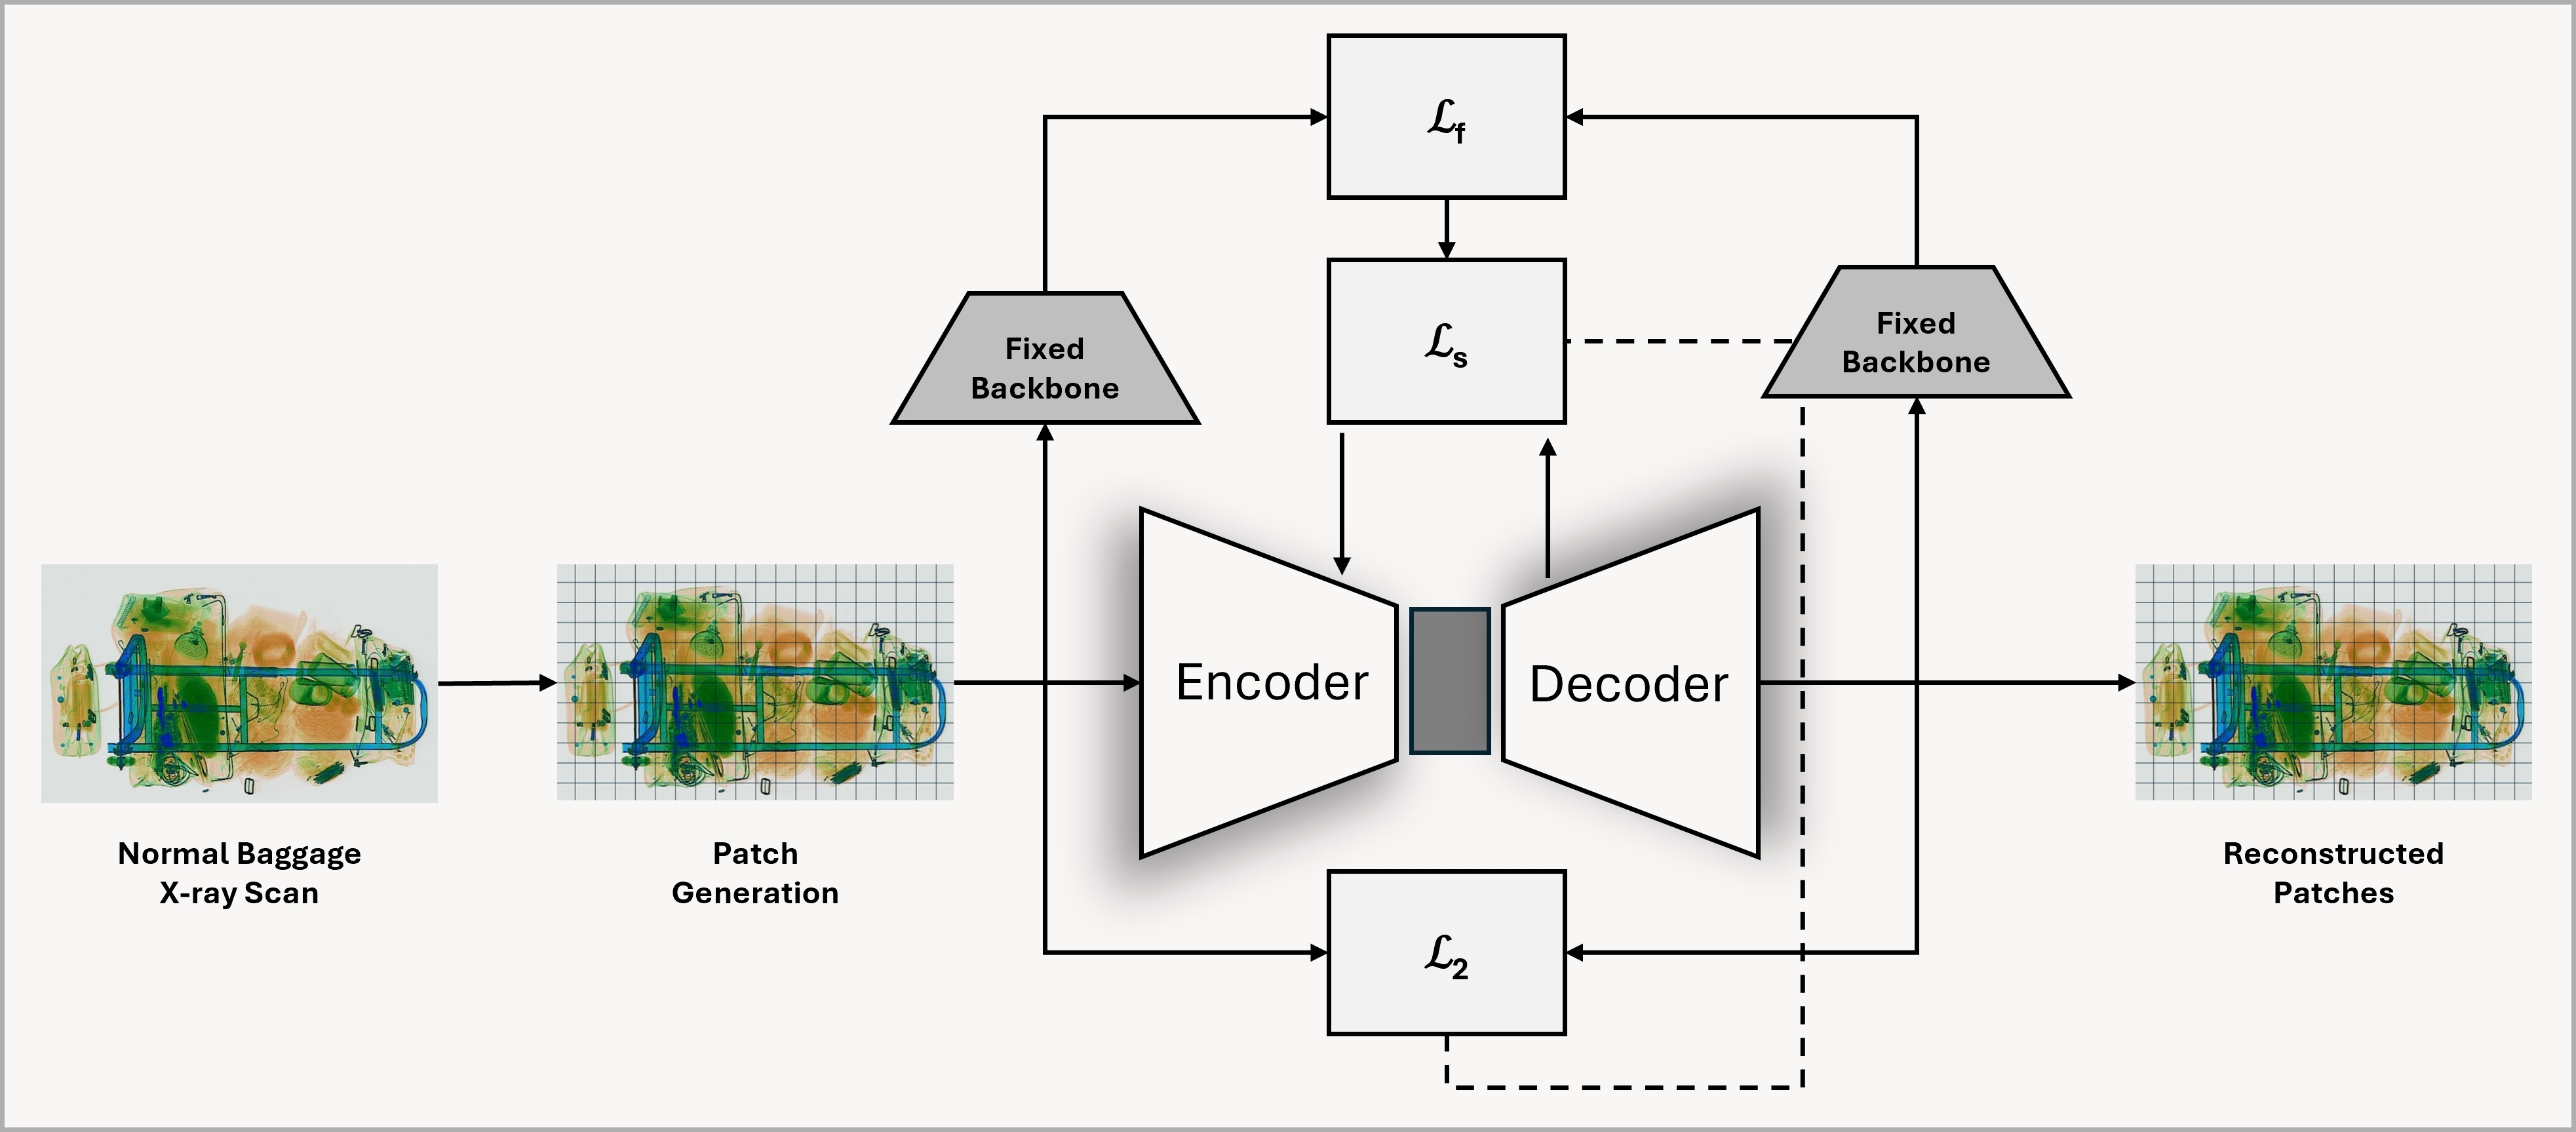
\includegraphics[width=0.9\linewidth]{images/enc-dec.png}

\caption{Autoencoder training}
\label{fig:autoencoder}
\end{figure*}

\textbf{Training objective.} A key design choice is the use of a combined loss function that jointly optimizes pixel level fidelity and perceptual feature similarity:

\begin{equation}
\mathcal{L}_s = \alpha_1 \mathcal{L}_f + \alpha_2 \mathcal{L}_2
\end{equation}

The first term, $\mathcal{L}_f$, is a feature level loss computed in the space of a pretrained feature extractor $f(\cdot)$, measuring the mean absolute difference between the feature representations of the original and reconstructed images across a batch of size $b_s$:

\begin{equation}
\mathcal{L}_f =
\frac{1}{b_s}
\sum_{i=1}^{b_s}
\left| f(k_i) - f(k'_i) \right|
\end{equation}

The second term, $\mathcal{L}_2$, is a pixel wise mean squared error between the original image $k_i$ and its reconstruction $k'_i$:

\begin{equation}
\mathcal{L}_2 =
\frac{1}{b_s}
\sum_{i=1}^{b_s}
\left| k_i - k'_i \right|^2
\end{equation}

The weighting coefficients $\alpha_1$ and $\alpha_2$ balance the contribution of each term. This combined loss is critical: $\mathcal{L}_2$ alone tends to produce blurry reconstructions that lose high frequency details, while $\mathcal{L}_f$ enforces structural and perceptual consistency. Together, they produce reconstructions that are faithful to normal imagery while remaining sensitive to subtle anomalous structures such as small metallic objects embedded in cluttered baggage.

\textbf{Disparity Map Computation:}
At inference time, for an input image $I$, the CAE produces a reconstruction $R$. The disparity map $D$ is computed as the per pixel absolute difference:

\begin{equation}
D(x,y) = \| I - R \|
\end{equation}

This map assigns high values to regions where the model's reconstruction deviates from the input, the spatial signature of anomalous content. It forms the input signal to both downstream stages.

\subsection{Feature Extraction and Image Level Classification}

While the raw disparity map encodes spatial anomaly information, feeding it directly to a classifier would be high dimensional and noisy. Instead, a compact set of statistical features is extracted from $D$ to produce a fixed length descriptor for downstream classification.

\textbf{Feature extraction.} Features are derived from the disparity map to capture both global reconstruction error magnitude and local spatial structure. These include global statistics (mean, standard deviation, maximum, and upper percentile values of $D$), spatial concentration metrics (the proportion of pixels exceeding an error threshold), histogram based distribution descriptors, and regional block statistics capturing localized error patterns that may correspond to small threat objects. The resulting feature vector compactly summarizes the anomaly signal in a form suitable for classical machine learning, while preserving interpretability and robustness under limited labeled data.

\textbf{Classifier selection.} The extracted features are used to train a Random Forest classifier, selected following empirical comparison against Extreme Gradient Boosting (XGBoost) and Logistic Regression on the same feature set. As shown in the table, the Random Forest achieved the highest performance across all metrics, reaching an accuracy of 0.82–0.99, an F1 score of 0.42–0.62, and a ROC-AUC of 0.85–0.92. Its robustness to feature scale heterogeneity, native handling of class imbalance through class weight adjustment, and strong generalization under limited anomaly labels make it well suited to this setting. The ensemble comprises 200 decision trees, with class weights set inversely proportional to class frequency to compensate for the severe imbalance between normal and anomalous samples in the SIXray dataset.

\begin{table}
\begin{center}
\begin{tabular}{|l|c|c|c|}
\hline
Model & Accuracy & F1 & ROC-AUC \\
\hline\hline
Random Forest & 0.82 -- 0.99 & 0.42 -- 0.62 & 0.85 -- 0.92 \\
Extreme Gradient Boosting & 0.74 -- 0.84 & 0.32 -- 0.44 & 0.76 -- 0.79 \\
Logistic Regression & 0.81 -- 0.87 & 0.30 -- 0.40 & 0.90 -- 0.91 \\
\hline
\end{tabular}
\end{center}
\caption{Classification performance comparison across different models.}
\label{tab:results}
\end{table}

\subsection{Patch Wise Localization via Connected Component Analysis}

Image level detection indicates whether a threat is present but provides no spatial guidance. When the classification stage flags an image as anomalous, the localization stage is activated to identify the precise region of interest.

\textbf{Patch wise reconstruction.} Rather than analyzing the full image reconstruction holistically, the localization stage operates at fine spatial granularity. The input image is upscaled to $2240\times2240$ pixels and partitioned into non overlapping tiles. Each tile is independently reconstructed by the CAE, producing a tiled disparity map that retains high spatial resolution across the full image extent. This patch wise strategy allows the model to isolate reconstruction errors to small sub regions, which is critical for detecting compact threat objects that would otherwise be diluted in a global analysis.

\textbf{Localization pipeline.} The spatial anomaly signal is refined through the following sequence of operations:

\textbf{Step 1 -- Disparity Computation:}
The disparity map

\begin{equation}
D(x,y) = \| I - R \|
\end{equation}

is computed from the tile wise reconstructions, producing a high resolution map of reconstruction error across the image.

\textbf{Step 2 -- Thresholding:}
A binary mask $M$ is obtained by applying a threshold $T$:

\begin{equation}
M(x,y) =
\begin{cases}
1, & \text{if } D(x,y) > T \\
0, & \text{otherwise}
\end{cases}
\end{equation}

The threshold $T$ is optimized on the validation set by sweeping candidate values and selecting the one that maximizes localization F1 at IoU $\geq 0.3$.

\textbf{Step 3 -- Connected Component Extraction:}
Connected component analysis (CCA) is applied to the binary mask $M$ to identify spatially contiguous regions of elevated reconstruction error. Each connected component represents a candidate threat region.

\textbf{Step 4 -- Component Filtering:}
Components are filtered by size, retaining only those whose area falls within a predefined range $[min\_size, max\_size]$. This removes both noise induced micro components and large background artifacts that are unlikely to correspond to localized threats.

\textbf{Step 5 -- Bounding Box Generation:}
Each surviving component is enclosed in a padded bounding box, projected back to the coordinate space of the original image, and returned as the localization output.

The hyperparameters $T$, $min\_size$, and $max\_size$ are each tuned independently on the validation set. This post processing pipeline transforms the continuous disparity signal into discrete, interpretable bounding regions, directly actionable by human screening operators.

\subsection{Design Rationale}

Three principles guided the framework's design:

\begin{itemize}
    \item \textbf{Label efficiency:} The CAE requires no anomaly annotations during training, and the RF classifier requires only image-level labels rather than pixel-wise segmentation masks.
    
    \item \textbf{Modularity:} The classification and localization stages are decoupled and can be updated independently. For instance, the RF could be replaced with a neural classifier as labeled data accumulates, without retraining the CAE.
    
    \item \textbf{Computational practicality:} Both the feature extraction and Random Forest inference are lightweight, and the CAE architecture is kept shallow enough for deployment in time-constrained security screening environments without GPU dependency at inference time.
\end{itemize}

\section{Template}

\subsection{Paper length}
Papers must not exceed 14 pages (excluding references). References and any appendices are unlimited.
{\bf Only}  the acknowledgement and bibliography should be {\em excluded} from the page count: Papers must not have altered margins and formatting from those laid down by this style guide.

The bibliography should begin immediately after the paper text.  It may
be of any length, within reason.  It must {\em not} include
annotations, figures, or any other paraphernalia intended to subvert the
paper length requirement.

\subsection{Citations}
When citing a multi-author paper, you may save space by using ``{\em et
alia}'', shortened to ``\etal'' (not ``{\em et.\ al.}'' as ``{\em et}'' is
a complete word.)  The provided \verb'\etal' macro is a useful {\em aide
memoire} in this regard.  However, use it only when there are three or more
authors.  Thus, the following is correct: `` Frobnication has been trendy
lately.  It was introduced by Alpher~\cite{Alpher02}, and subsequently
developed by Alpher and Fotheringham-Smythe~\cite{Alpher03}, and Alpher
\etal~\cite{Alpher04}.''

This is incorrect: ``... subsequently developed by Alpher \etal~\cite{Alpher03} ...''
because reference~\cite{Alpher03} has just two authors.  If you use the
\verb'\etal' macro, then you need not worry about double periods
when used at the end of a sentence as in Alpher \etal.

%For this citation style, keep multiple citations in numerical (not
%chronological) order, so prefer
We use {\tt natbib}, so citations in random order are nicely sorted:
 \cite{Alpher03,Alpher02,Authors06b,Authors06}.  However, we don't use the
compress option, as we want each reference to have its own hyperlink and
popup window.

%-------------------------------------------------------------------------
\subsection{Footnotes}

Please use footnotes\footnote {This is what a footnote looks like.  It
often distracts the reader from the main flow of the argument.} sparingly.
Indeed, try to avoid footnotes altogether and include necessary peripheral
observations in
the text (within parentheses, if you prefer, as in this sentence).  If you
wish to use a footnote, place it at the bottom of the column on the page on
which it is referenced. Use Times 8-point type, single-spaced.


\begin{figure*}
\begin{center}
\fbox{\rule{0pt}{2in} \rule{.9\linewidth}{0pt}}
\end{center}
   \caption{Example of a short caption, which should be centered.}
\label{fig:short}
\end{figure*}

\begin{table}
\begin{center}
\begin{tabular}{|l|c|}
\hline
Method & Frobnability \\
\hline\hline
Theirs & Frumpy \\
Yours & Frobbly \\
Ours & Makes one's heart Frob\\
\hline
\end{tabular}
\end{center}
\caption{Results.   Ours is better.}
\end{table}

\subsection{Mathematics}

Please number all of your sections and displayed equations.  It is
important for readers to be able to refer to any particular equation.  Just
because you didn't refer to it in the text doesn't mean some future reader
might not need to refer to it.  It is cumbersome to have to use
circumlocutions like ``the equation second from the top of page 3 column
1''.  (Note that the ruler will not be present in the final copy, so is not
an alternative to equation numbers).  All authors will benefit from reading
Mermin's description~\cite{Mermin89} of how to write mathematics.


%-------------------------------------------------------------------------
\subsection{References}

List and number all bibliographical references in 9-point Times,
single-spaced, at the end of your paper. When referenced in the text,
enclose the citation number in square brackets, for
example~\cite{Authors06}.  Where appropriate, include the name(s) of
editors of referenced books.


%------------------------------------------------------------------------
\subsection{Color}

Color is valuable, and will be visible to readers of the electronic copy.
However ensure that, when printed on a monochrome printer, no important
information is lost by the conversion to grayscale.

\bibliography{egbib}
\end{document}